\section{Exercício 12}

    Fazer um programa que gere os \emph{n} primeiros números da sequência de
    Fibonnacci, e armazene a sequências em endereços consecutivos a partir da
    posição de memória com rótulo idx. Esta operação deve ser feita com uma
    chamada de função para o rótulo SeqFibonnacci.  

\subsection{Descrição Alto Nível}

A desrição em alto nível foi utilizando a linguagem python é desta forma:

\begin{lstlisting}

def fib(n):
    a, b, c = 0, 1, 0
    res = []
    while c < n:
        res[a] = b
        a, b = b, a+b
        c+=1

\end{lstlisting}

\subsection{Descrição Baixo nível}
\begin{verbatim}
    
.CODE
INIT:	
	lda #0
	sta n1
	lda #1
	sta n2
	lda p
	add #2
	sta p
	lda n
	add #-2
	sta n
	LOOP:
		jz	FIM
		jsr SEQFIBONACCI
		lda	p
		add	#1
		sta p
		lda n
		add	#-1
		sta	n
		jmp LOOP
			SEQFIBONACCI:
				lda n1
				add n2
				sta nxt
				sta p,I
				lda n2
				sta n1
				lda nxt
				sta n2
				rts     
FIM:
	hlt
                     
.ENDCODE

.DATA
    n:      db  #10      ;Seq FIB
    n1:     db  #0		 ;fib-2
    n2:     db  #0		 ;fib-1
    nxt:    db  #0		 ;n1 + n2
    p:      db  #idx
    idx:    db  #0, #1, #0, #0, #0, #0, #0
.ENDDATA

\end{verbatim}

\subsection{Tela Montador}

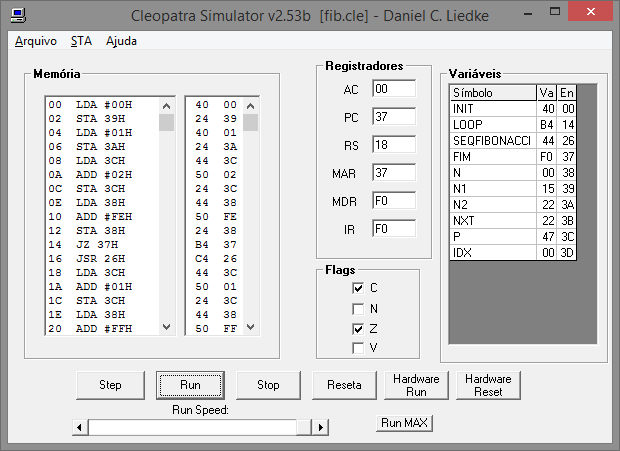
\includegraphics{images/fib.png}

\subsection{Contagem Operações e estimativa de de tempo de execução}

Considerando \emph{n} como \emph{x} temos a seguinte função:
$$f(x) = 124x + 65$$
O Tempo de excução seria xxx ao considerarmos que o Cleópatra opera a
1GHz.

